\section{Narvis: System Design and Implementation}

% Thus, it has two kinds of users: editors, the data visualization experts who use Narvis to create an explanation slideshow, and audiences, the general audience who watch the slideshow created by ediors.

Guided by the theory model discussed in section3, as well as the design consideration mentioned in section 4, we desing and implement Narvis, an authoring tool for crafting slideshows for the presentation of visualization. The workflow of Narvis consists of three phases (Figure \siwei{ref}), i.e., Automatic Analysis Phase, Manual Editing Phase, and Viewing Phase.

% The workflow of Narvis includes three phases (Figure \siwei{ref}):  In Automatic Analysis Phase, the system accepts the input visualization, extracts graphical elements and classifies them into groups for further edit. 
% In Human Editing Phase, editors will be involved to modify the output from the Automatic Analysis Phase, and use the templates Narvis provide to craft a explanation slideshow. 
% In Reviewing Phase, audience can assess the slide show generated in Human Editing Phase. Their click activity and comments will be recorded and send to the editors, helping them improve the quality of the slide show. 

\begin{figure}
 \centering % avoid the use of \begin{center}...\end{center} and use \centering instead (more compact)
 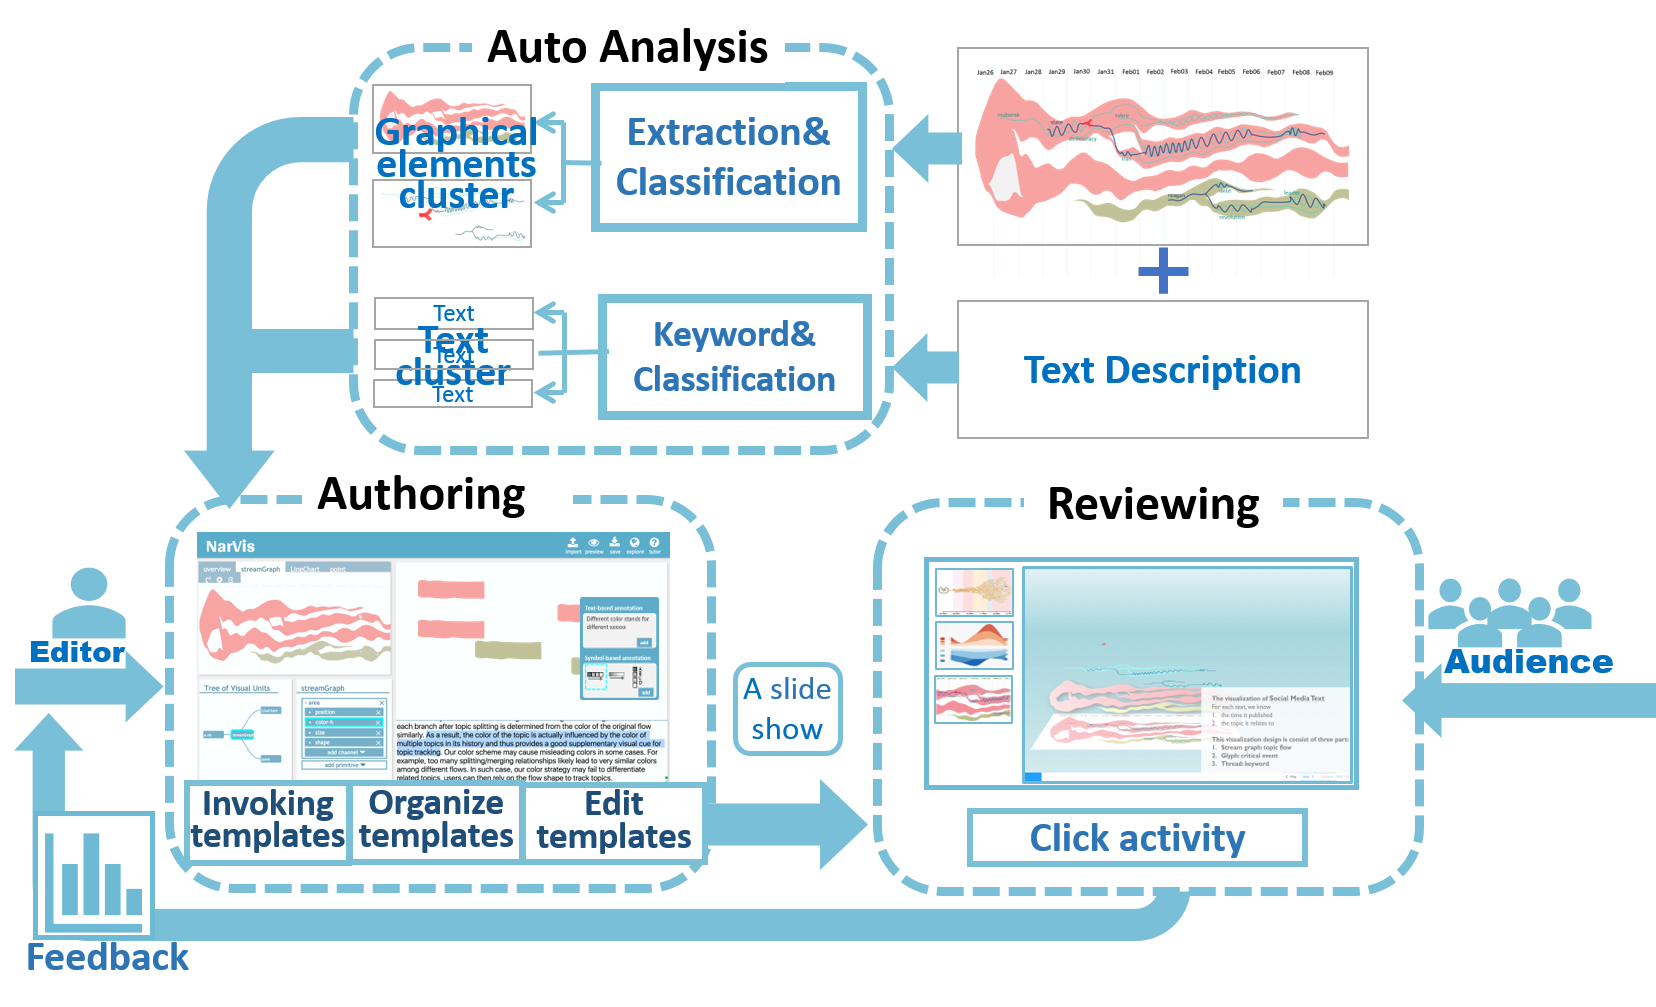
\includegraphics[width=\columnwidth]{overview}
 \caption{The system overview}
 \label{fig:overview}
\end{figure}

\subsection{Phase1: Auto Analysis}

% The auto analysis has two parts: one for input image and one for input text. It automatically extract the graphic elements and divide them into different cluster, facilitating later editing.(DE1) Note that the textual input is not necessary but it provides hints when editors add annotations manually in the Human Editing Phase.(DE1)

The input of Narvis includes two parts: one image presenting a visual design (mandatory) and a piece of text describing the design (optional). Here, we explain the basic idea of how Narvis analyze these input source to facilitate further authoring. 

\subsubsection{Analysis of Input Image}
% The auto analysis of input image has three main steps. It first detects all primitives that it finds in the given image and also detects any labels that are present in the visualization. It will then cluster objects that are spacially linked and extract non-target objects. Finally, it will fill in any empty spaces left inside objects from extraction with the appropriate color so as to show the target object in its entirety.
The analysis of input image includes two steps, object detection and object clustering.
% and object recovery.

% The first step, object detection, is done by iterating through all the pixels on the bitmap. 
\noindent
\textbf{Object detection.} We iterates through all pixels, and clusters all the pixels that are i) neighbors and ii) have the similar color through a modified Breath-first search algorithm(see in Algorithm~\ref{alg:alg1}). Simple objects, such as a bar in a bar chart, a node in scatter plot, are detected and extracted after this step.

\noindent
\textbf{Object clustering.} All the objects with spatial and appearance similarity are clustered to allow an efficient manipulation, as described in Algorithm~\ref{alg:alg2}. For example, all the nodes in a scatter plot should be put in one cluster, instead of letting the editor add them one by one manually.     
%\noindent 
%\textbf{Object recovery.} Once we have completed extraction, we have the issue of these white spaces. The reason this is an issue is because an extracted object might have been dividing two objects, and so when it is extracted, we lose the boundary between our target object and another object, which can cause confusion as to whether that white space should be colored in or not. To solve this boundary problem, we create a queue of the white spaces, with each data point giving the starting and ending point of that space. We then look at the intervals between enclosed white spaced objects, if that interval is above a threshhold, we take that white space to not be part of our object. If it is below our threshhold, then we enclose the white space with the target objects color, creating a boundary for it. The main difference is that for objects not within our target object, we do not create a boundary, whereas objects within our target object are enclosed with the target objects color.

\subsubsection{Analysis of Input Textual Description}
For the input textual description, we offer a basic text detection and classification algorithm, which is based on a dictionary of terms that are identified as highly correlated with visual grammars. E.g. the word ``length'' and ``encodes with'' ,are highly correlated with the  visual grammar of size. We extract all the sentences containing the terms in our dictionary, and cluster them based on the terms they have.

The algorithm we proposed is a compromise between efficiency and performance. At this time point, it is limited to images with high quality and clear edges, but its performance can be improved by adopting other well-established algorithm, such as the algorithm based on patch detection and clustering \cite{savva_revision:_2011} and the algorithm based on edge maps \cite{huang2003model}.

\begin{algorithm} 
        \caption{Object Detection}  
        \label{alg:alg1}
        \begin{algorithmic} % line number
            \Require A bitmap in the form of a two-dimensional array: $A$
            \Ensure A list of objects: $B$
            \State $B \gets \{\}$
            \ForAll{$pixel (x,y) \in A$} 
                \If{no mark on $pixel(x,y)$}
                    \State $Q \gets \{(x,y)\} $
                    \State $Obj \gets \{\}$
                    \ForAll{$(x,y) \in Q$}
                        \State $Q = Q - \{(x,y)\}$
                        \State $Obj = Obj \cup \{(x,y)\}$
                        \ForAll {$(x',y')$ which $|x'-x|+|y'-y|\leq2$ and no mark on $pixel(x',y')$}
                            \If{$pixel(x,y)$ and $pixel(x',y')$ have similar color}
                                \State $Q = Q \cup \{(x',y')\}$
                                \State Make a mark on $(x',y')$
                            \EndIf
                        \EndFor
                    \EndFor
                    \State $B = B \cup \{Obj\}$
                \EndIf
            \EndFor
            \State \Return{$B$}
        \end{algorithmic}  
    \end{algorithm} 
    
    
    \begin{algorithm}  
        \caption{Object Clustering} 
        \label{alg:alg2} 
        \begin{algorithmic} % line number
            \Require A list of objects: $A$, the number of clusters: $N$
            \Ensure A list of objects: $B$
            \State $E \gets \{\}$
            \ForAll{$a_1 \in A$}
                \ForAll{$a_2 \in A$ and $distance(a_1,a_2) \leq L$} \Comment{$L$ is a parameter that accelerates our calculations}
                    \If{$a_1$ and $a_2$ have similar color}
                        \State $d \gets$ the distance between $a_1$ and $a_2$
                        \State $E \gets E \cup \{(a_1, a_2, d)\}$
                    \EndIf
                \EndFor
            \EndFor
            \State $B \gets A$
            \State $E \gets$ sort $E$ by the $d$ of each elements in descending order
            \ForAll{$(a_1,a_2, d) \in E$}
                \State $b_1 \gets b|b\in B, a_1 \subseteq b$
                \State $b_2 \gets b|b\in B, a_2 \subseteq b$
                \If{$b_1 \neq b_2$}
                    \State $B = (B - \{b1\} - \{b2\})\cup \{b1 \cup b2\}$
                \EndIf
                \If{$|B|\leq N$}
                    \State break
                \EndIf
            \EndFor
            \State \Return{$B$}
        \end{algorithmic}  
    \end{algorithm} 

\subsection{Phase2: Authoring}
In Narvis, editors craft an introduction slideshow by constructing build-in blocks called as templates in Narvis. We first introduce the workflow of this phase, which includes three steps, i.e., invoking templates, organizing templates and modifying templates, as illustrated in Figure~\ref{fig:overview}. Then ,we explain how we design and organize the templates in Narvis. 
% We introduce three panels in this phase acting as three steps in the workflow to allow editors  

\subsubsection{Invoking Templates} 

After graphical elements are extracted and clustered based on visual representation, each cluster appears as a tabbed panel in the \textit{Source Panel} (Figure \siwei{ref}). 

Editors can switch between these tabbed panels, add or delete graphical elements in each panel, making sure that 1) all the graphical elements of the same visual unit is in the same panel 2) every graphical element belongs to one and only panel. Then, for each visual unit, the user call a template from all the templates provided by Narvis. For example, for the tabbed panel in \siwei{fig}, the editor should call a ``scatter plot'' template.


The relationship between graphical elements and templates is similar to the one between data and function. Templates contain a set of operations to produce a sequence of slides from the input graphical elements.  (DE1, DE2) \siwei{I do not understand this paragraph, too abstract}

\subsubsection{Organizing Templates} 
Once invoked, a template will show on the \textit{Tree Panel} as a tree node. 
By dragging and dropping these nodes, editors organize the structure of the tree diagram, which reflects the relationship between visual units and determines the narrative sequence of the slideshow.(DA5) 

\subsubsection{Modifying Templates} 
% \textbf{\textit{ Unit Panel \& Editor panel}: personalized modification}
% but it also allow the users high flexibity to modify these temples, thus guaranteeing the expressiveness of this system. 
Narvis provides templates to generate slideshows with high efficiency. 
It also supports flexible modification of templates for expressiveness.
Editors can edit a template in the \textit{Unit Panel} by selecting a node on the \textit{Tree Panel}. In each template, all possible visual grammar are enumerated. Editors can unused one themselves, instead of adding the ones used, thus eliminating the unconscious omission of crucial information (DA.5).\siwei{now? } 
It also recommends a narrative sequence of visual grammars, based on the metrics we mentioned in section 3.1.4 (DE1, DA3, DA5). 
In the \textit{Editor Panel} \siwei{refer to the figure of interface when introducing Panels.}, with the hints from Narvis, editors add annotations to facilitate graph and chart comprehension. For each slide \siwei{the advant of slide is strange. what is the relationship between slide, templates, and visual grammar? Please clarify in advanced.}, Narvis offers questions or sentence with blank for adding text-based annotation and a list of suggested design options for symbol-based annotation. \siwei{Can you give an example? It is hard to follow.}

\subsubsection{A Library of Templates}
\siwei{this subsubsection can be move to the first subsubsection. otherwise the library you mentioned does not make sense.}
We propose a library of templates for the narrative explanation of a visualization. A template is a set of slides that tends to introduce an visual unit. Since advanced visualization design is the assembly of miscellaneous visual units, such templates can achieve a high level of efficiency for the explanation of a visualization (DA1). Furthermore, to adapt to various usage scenario, Narvis allows users to modify and refine templates through rich interactions.

\noindent
\textbf{Types of templates.}
Narvis use a 8*3 \siwei{what are eight rows and three columns?} table to organize the provided templates, as shown in \textbf{fig}. Narvis is extensible, new templates can be added by its developer through programming, or by end users through uploading their modified templates. At the same time, all newly added templates are classified into a certain cell of the 8*3 matrix \siwei{how to you classify a user-defined template?}, so as to avoid overwhelming users with a cornucopia of confusing options.

\noindent
\textbf{Templates design.}
We apply the analysis and theory model in section 3 \siwei{use ref rather than a direct number for reference.} for the design of templates. A template has four core components: 1) a well-considered narrative sequence for visual grammar explanation; 2) exaggeration or suppression of certain visual channels in some slides; 3) a series of narrative techniques such as attention cues, animated transitions, information repetition, to orientate visual attention and facilitate perception (DE.1); 4) Hints for adding annotations (DE.2) in each slide (DA.4) 

With a visual unit, more specifically, a set of graphic elements, as input, a templates will generate a slideshow and each slide illustrates one visual grammar(DA.4). \siwei{move DA.4 before dot, and check all these reference} These slides are sorted based on the narrative sequence we discussed in section 3.3. In each slide, we offer hints to guide the annotation process. These hints are sentence with blanks to fill in, heuristic questions, or a list of suggestion symbols. A visual channel is suppressed until its grammar has been explained. For example, before we introduce the visual grammar of color, all the object will be gray.  The graphical elements in different slides, which might have different visual appearance due to the applied exaggeration or suppression of visual channels, are perceptively connected through morphing animation. \siwei{try to explain it using a figure. Otherwise, it is hard to follow.}

\noindent
\textbf{Animation embedded in templates }

Narvis provides 8 types of animation, implement them in templates based on their effects on human attention and perception(DA.1) \siwei{add a space before `(', check this problem in the whole paper}, which has been widely discussed in previous work.\cite{robertson_effectiveness_2008, waldner_attractive_2014, heer_animated_2007} \siwei{typesetting problem, check it in the whole paper} We also provide a novel decomposition animation at the beginning of the introduction slideshow to engage the audience as well as to help them get a sense of overview.(DA.6) \siwei{it is not clear how animation relates to DA6}
\original{Animation is a double-edge sword, which introduces both benefits and pitfalls. We are not discussing the effects of animation here.} \siwei{Keep your sentence simple. I would suggest: Animation is optional} Editors can choose to remove these animation if they prefer an abstract slide show or they are suspicious of the effects of animation. 

\begin{table}[tb]
  \caption{A summary of animation provided}
  \label{tab:animation}
  \small
  \centering
  \begin{tabular}{p{1cm}|p{0.9cm}|p{0.9cm}|p{0.9cm}|p{1.5cm}|p{0.9cm}}
  \toprule
 \textbf{Animation} &\textbf{Engaging} & \textbf{orientate attention} & \textbf{perception} &\textbf{working scenario} &\textbf{ref} \\ 
  \midrule
  \textbf{Morphing} &\checkmark & \checkmark &\checkmark & grammar of size, grammar of shape & \cite{ruchikachorn_learning_2015, heer_animated_2007} \\ 
  \midrule
  \textbf{Blur} &   &\checkmark  &   & focus+context & \cite{pinto2008selecting}\\ 
 \midrule
  \textbf{Flicker} & & \checkmark &  & focus &\cite{waldner_attractive_2014} \\
  \midrule
  \textbf{Motion} & \checkmark & \checkmark & \checkmark & grammar of position & \cite{huber_visualizing_2005} \\
  \midrule
  \textbf{Zoom-in/out} & \checkmark &\checkmark &  & focus&  \\
  \midrule
  \textbf{Annotation} &  & \checkmark &\checkmark &   textual explain & \cite{segel_narrative_2010 } \\
  \midrule
  \textbf{Fade in/out} &  & \checkmark &  & & \\
  \midrule
  \textbf{Decompose} & \checkmark &  &\checkmark & Show how a visualization is composed by visual units & A novel design by us \\
  \bottomrule

  \end{tabular}
  \vspace{1mm}
\end{table}

\subsection{Phase3: Viewing}
By clicking the ``explore'' icon on the right top, audience will be directed to reviewing mode and watch the slideshow produced in Narvis.
\subsubsection{The Interface for Audience}
The interface of audience is composed of two panels.

\noindent
\textbf{\textit{Gallery Panel:} the collection of generated slide show.} \siwei{introduce interface with figure reference.}
\textit{Gallery Panel} exhibit all the slideshows produced by editors and saved in Narvis. Every slideshow \siwei{do you mean slide?} is presented by an image, the visualization it tends to explain. By clicking on the image, users can watch this slideshow in the \textit{Screen Panel}. 

\noindent
\textbf{\textit{Screen Panel:}  review and comment}
Every slideshow displayed in \textit{Gallery Panel} is a series of slides, each of which is responsible for the delivery of one visual grammar. In the \textit{Screen} panel, users click buttons to move forward or backward to view these slides, and their click activity will be recorded automatically by Narvis. 

\subsubsection{Generated Report}
The report visualizes the click activity of audience in the form of a stacked bar chart, as\textbf{fig}. The heigh of the bar indicates the time spent on watching this slide. If audiences go back to a previous slide while viewing, a bar will be stacked on the top of the previous one. If there are animation in the slide show, a white line will be drawn upon the bar chart, referring to the animation playing time of each slide, thus gives a judgement whether an animation is too fast or too slow. (DE.3)

\subsection{Iterative Design}
To investigate the usability of Narvis, we invited 4 UGs \siwei{4 or 7? make it consistent with Section 3} from diverse backgrounds to watch an introduction slideshow produced by a data visualization professor with Narvis. 
Based on their feedback, we iterate over the design of Narvis as follow:

\subsubsection{An Compulsory Introduction}
In the initially design, an introduction slideshow is purely the combination of templates. In other words, it just explain each visual units after displaying an overview of the visualization. However, the participants complained that they are less motivated to learn a visual design without an awareness of the background. Questions like, \textit{what's the motivation of this visual design}, \textit{what's the dataset}, and \textit{what kinds of problems it can solve} need to be answered before the introduction of this visual design. Thus, we add a compulsory introduction slide at the beginning of each slideshow, which is displayed as a root node of the tree diagram in \textit{Tree Panel}. This slide contains questions that guide the editors to give a brief description of the background.
\subsubsection{Different Levels of Detail}
While 3 UGs appreciate this detailed introduction slideshow, and consider the animation applied as engaging and enjoyable. Another UG, who has taken a data visualization course before and is familiar with some visualization designs, thought some slides and animation are redundant. 
Thus, we offer 3 levels of details which the audience can choose from. The detailed one displays all the animation, the normal ones skip the animation for some simple visual grammar such as color and size, and the abstract one discards all animation and put the annotation for color and size in one slide
 
\begin{figure}
 \centering % avoid the use of \begin{center}...\end{center} and use \centering instead (more compact)
 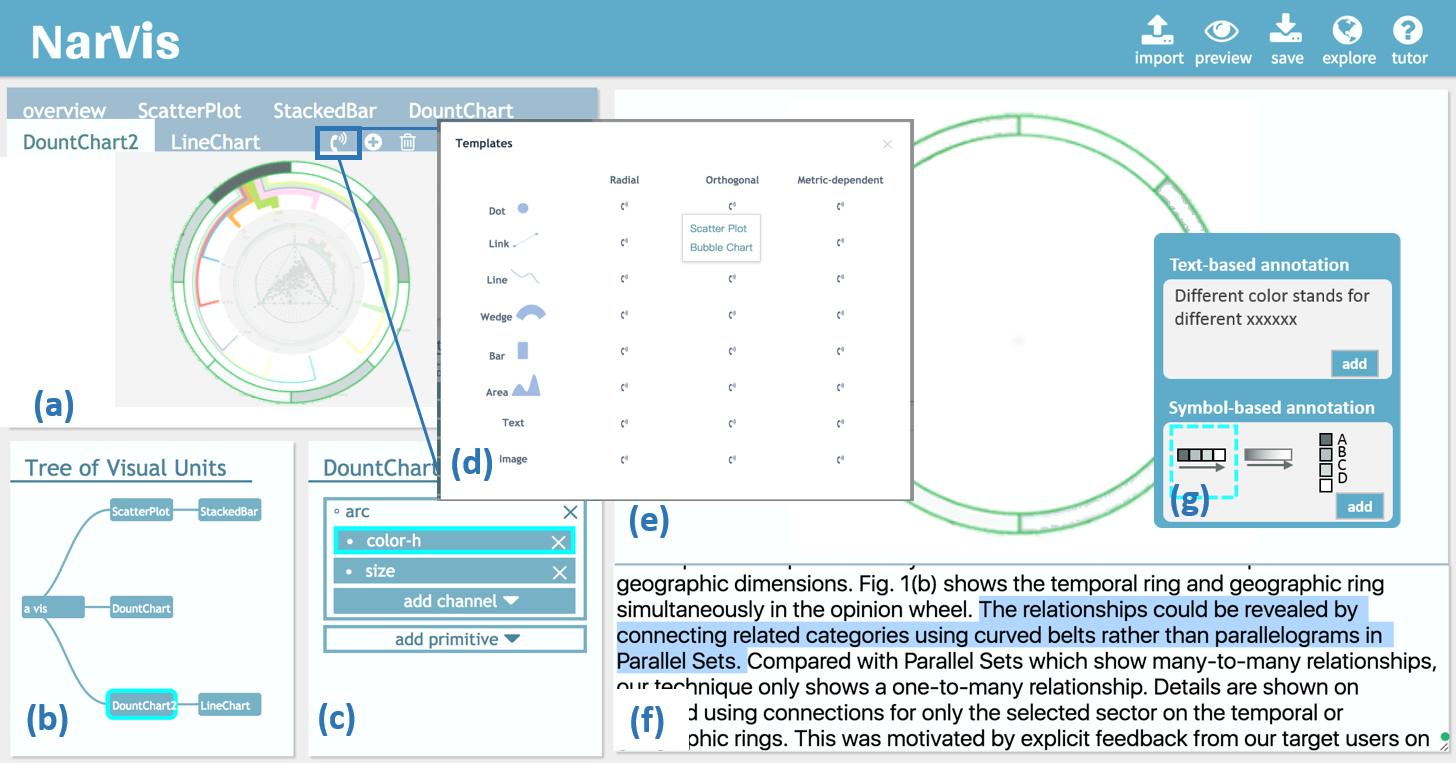
\includegraphics[width=\linewidth]{interface}
 \caption{Annotated screenshot of the interface of Narvis: a) Source Panel, b) Tree Panel, c) Unit Panel, d) the library of templates, e) Edit Panel, f) text area where the related sentence is highlighted from input textual description, g) a floating annotation window that offers options for adding annotation}
 \label{fig:interface}
\end{figure}

   
\subsection{A Working Scenario}
Jessica has extensive experience in the field of data visualization, and has implement a visual analytics tool in a review service website based on the design of OpinionSeer\cite{wu_opinionseer:_2010}, which has five visual units as demonstrated in Figure~\ref{fig:hierarchic}. To help audience better understand this design, she needs to publish a tutorial accompanied with it.
First, she loads the screen-shot of her system, as well a textual description, into Narvis.
After a few seconds, the system automatically extracts the graphics elements through an edge detection algorithm. Jessica first adds five tabbed panels in Figure~\ref{fig:interface}(c), since she identifies five differen visual units in OpinionSeer. At each panel, where the uploaded image shows with half-transparency as background, Jessica adds graphical elements by clicking it. As in Figure~\ref{fig:interface}(c)), the ``geometry ring'' is added to a tabbed panel and highlighted. Note that Narvis pre clusters some graphical elements to convenient the users. For example, all the dots in ``scatter plot'' will be highlighted just by clicking on one dot. 

After some editing, each tabbed panel includes all graphics elements belonging to one visual unit. Now, she chooses narrative templates for each visual unit. 
She first choose a visual unit by clicking its tab, then clicks the ``phone'' icon. A table Figure~\ref{fig:interface}(a) jumps up, which categorize all the templates as the 8*3 table we described in Figure~\ref{compositions}. For example, when Jessica clicks on the (2,1) cell, a dropdown list that contains two templates, Bubble chart and Scatter Plot, will appear.  

One by one, Jessica invokes 5 templates, all then show as tree nodes in \textit{Tree Panel}(see in Figure~\ref{fig:interface}(d)) as children of the ``a vis'' node. Jessica reorganizes the structure of the tree diagram (see in Figure~\ref{fig:interface}(d)) by dragging and dropping based on her understanding of this visual design. 

Moreover, Jessica edits the narrative templates based on her design. 
% In the templates, we enumerate all the possible visual encodings. 
She goes through all five templates in the \textit{Unit Panel}(see in Figure~\ref{fig:interface}(e)) by clicking the corresponding node in \textit{Tree Panel}, and deletes the visual channels with no encodings, such as the size in the template of scatter plot. 

Jessica further adds annotations at each slide with the help from an annotation window(see in Figure~\ref{fig:interface}(h)). This annotation windows offers some design options for adding text-based annotation as well as symbol based annotation.  The text area Figure~\ref{fig:interface}(g) also offer hints for the addition of annotation by highlight the corresponding textual description. 
% When adding annotation to a certain channel, the related text will highlight in the text area, aiming to offer a better user experience.   


To refine the readability of the tutorial, Jessica asks several friends, who have little experience in data visualization, to watch the tutorial before release. Narvis collects their viewing behavior from click activities, generates statistics results, and visualize it in the form of stacked bar chart(see in Figure~\ref{fig:interface}(b)) , which helps Jessica answer questions like \textit{``which slides do they skip?''}, \textit{``which slides do they review several times?''}, and \textit{``which slides do they stay for a long time?''} and adjust her slideshow accordingly. 
% These click sequence data provides cues for Jessica to strengthen and refine the readability of the tutorial. 

% revealing information such as, ,   



